\subsection{Product perspective}
The S2B will be used by two kinds of users: customers store owner.

\subsubsection{Customer}
The customer can create reservations for a desired store: such reservation is then inserted into a queue.\\This queue is managed in order to avoid overcrowding. To achieve this, statistics about visits' durations are exploited, taking also into account information that customers may provide (e.g. which department of the store they want to visit).\\
There are multiple types of reservations that can be requested:
\begin{enumerate}
	\item Immediate reservation: the costumer wants to queue up immediately to a store. He/she is also provided with an estimation of the time he has to wait before his/her turn.
	\item Future reservation: the costumer wants to book a future visit at a desired time and store.\\ When creating the reservation the customer can specify how long he/she intends to stay and which departments of the market he/she plans to go to, in order to provide a better plan. If he/she does not specify the duration the system can infer it using some statistic built on his/her previous visits. Then the customer will be provided whit the actual time he will be able to access the store (considering the bookings from other customers).
	\item On premise reservation: the customer is allowed to enqueue directly at the store. Each of them will provide a system to print tickets so that those who do not have access to the required technology for the previous options can still line up.\\These tickets contain a reservation number and an estimation of the waiting time before being able to enter.
\end{enumerate}
Customers who requested an immediate or a future reservation receive an alert when they need to depart to reach the store.
This alert is based on the location of the customer, so that the time needed to reach the store is taken into account.\\
Moreover immediate and future reservations can be deleted by who created them.\\
\subsubsection{Store owner}
The store owner can set the maximum occupation threshold for each of his stores, to avoid overcrowding.\\
He/she can also monitor the number of customers inside at any time and visualize statistics about the flow of clients and department occupation.
\begin{figure}[!htb]
\centering
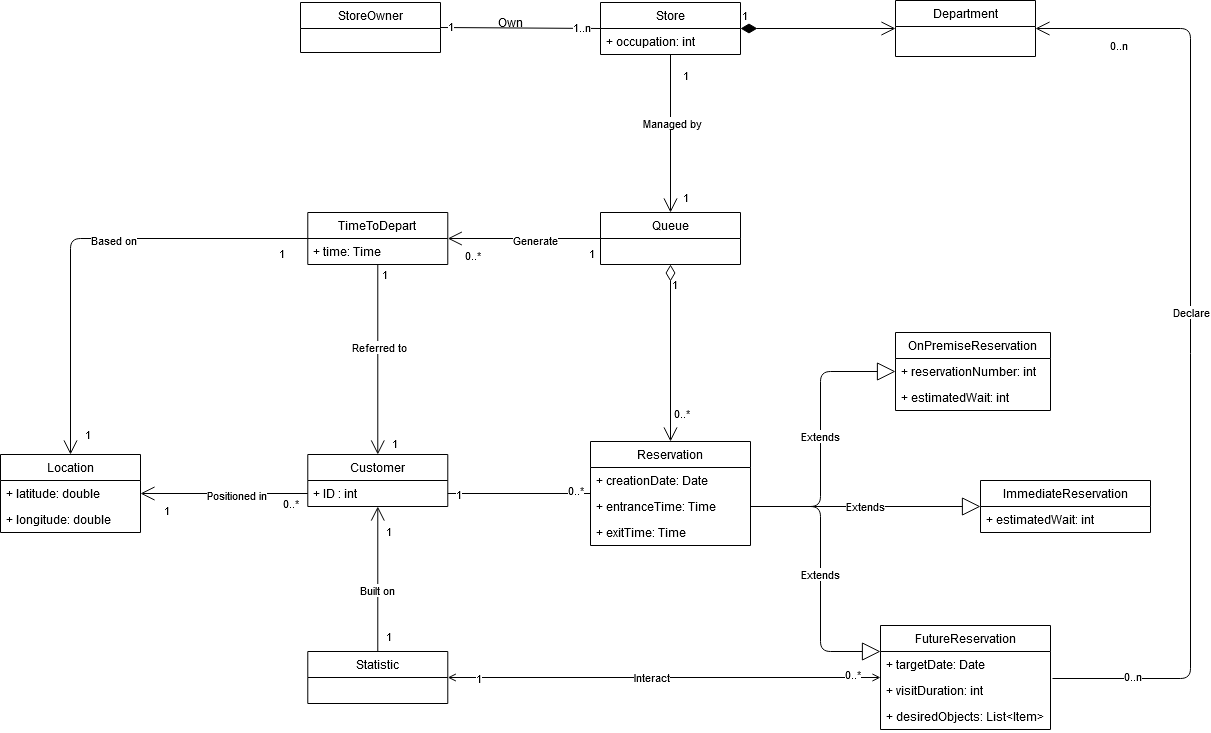
\includegraphics[width=\textwidth]{Images/ClassDiagram.png}
\caption{\label{fig:metamodel2}Class Diagram.}
\end{figure}
\subsubsection{State charts}
\begin{figure}[!htb]
	\centering
	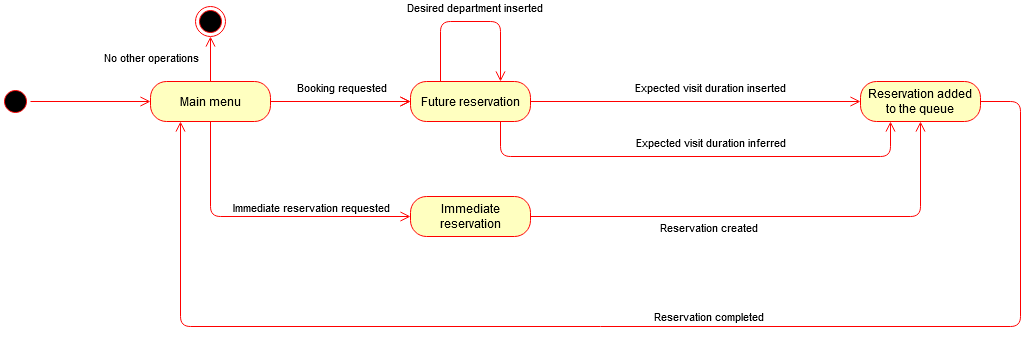
\includegraphics[width=\textwidth]{Images/StateDiagram.png}
	\caption{\label{fig:metamodel2}State Diagram 1: Creation of a reservation.}
\end{figure}
